\begin{align*}
    \polynomialQ{1}{N}{0} &= 0 \\
    \polynomialQ{1}{N}{1} &= 1 \\
    \polynomialQ{1}{N}{2} &= 6N - 4 \\
    \polynomialQ{1}{N}{3} &= 18N - 27 \\
    \polynomialQ{1}{N}{4} &= 36N - 80 \\
    \polynomialQ{1}{N}{5} &= 60N - 175 \\
    \polynomialQ{1}{N}{6} &= 90N - 324 \\
    \polynomialQ{1}{N}{7} &= 126N - 539 \\
    \polynomialQ{1}{N}{8} &= 168N - 832 \\
    \polynomialQ{1}{N}{9} &= 216N - 1215 \\
    \polynomialQ{1}{N}{10} &= 270N - 1700 \\
    \polynomialQ{1}{N}{11} &= 330N - 2299 \\
    \polynomialQ{1}{N}{12} &= 396N - 3024 \\
    \polynomialQ{1}{N}{13} &= 468N - 3887 \\
    \polynomialQ{1}{N}{14} &= 546N - 4900 \\
    \polynomialQ{1}{N}{15} &= 630N - 6075 \\
    \polynomialQ{1}{N}{16} &= 720N - 7424 \\
    \polynomialQ{1}{N}{17} &= 816N - 8959 \\
    \polynomialQ{1}{N}{18} &= 918N - 10692 \\
    \polynomialQ{1}{N}{19} &= 1026N - 12635 \\
    \polynomialQ{1}{N}{20} &= 1140N - 14800
\end{align*}
\begin{figure}[H]
    \centering
    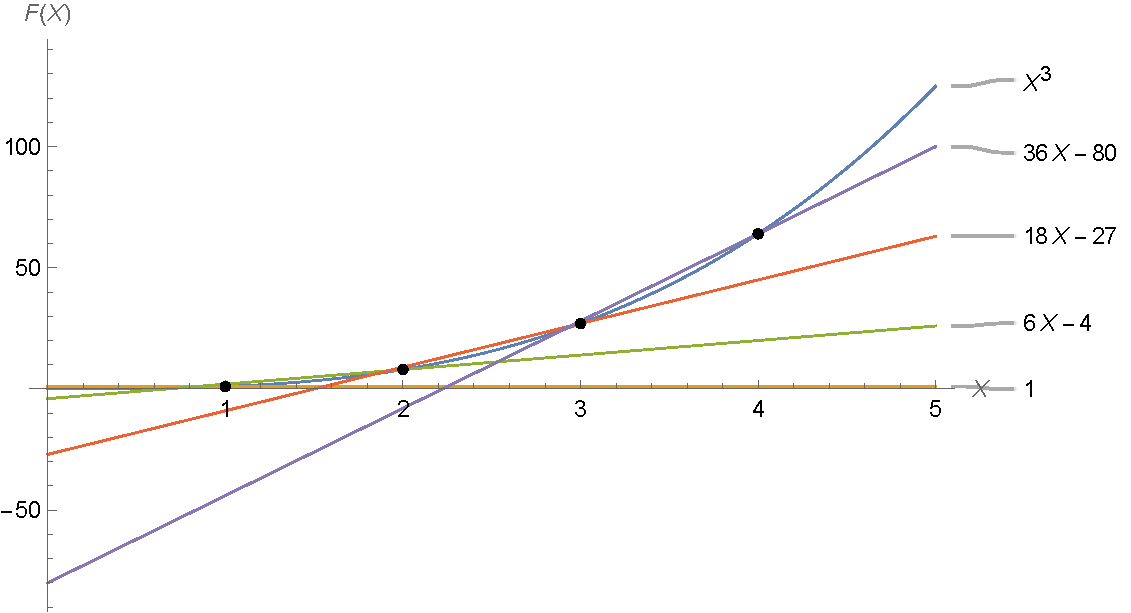
\includegraphics[width=1\textwidth]{sections/images/02_cubes_with_q_1_n_k}
    ~\caption{Polynomials Q(1, n, k)}\label{fig:figure2}
\end{figure}

